\documentclass[a4paper,12pt]{article}
\usepackage[utf8]{inputenc}
\usepackage[legalpaper, margin=0.5in]{geometry}
\usepackage{graphicx}
\usepackage{amsmath}

\setlength{\parindent}{0em}
\setlength{\parskip}{1em}

\graphicspath{{resources/}}

\title{Week 3: Computing Taylor Series}
\author{Jinil Jang }
\date{November 2019}

\begin{document}

\maketitle

\section{To compute the Taylor series}

\subsection{$\frac{1}{x}\sin{x^2}$}
\begin{equation}
\begin{split}
\frac{1}{x}\sin{x^2} & = \frac{1}{x}((x^2)-\frac{1}{3!}(x^2)^3 + \frac{1}{5!}(x^2)^5- \cdots) \\ 
 & = x - \frac{1}{3!}x^5 + \frac{1}{5!}x^9 - \cdots \\
 & = x^{-1}\Sigma_{k=0}^\infty (-1)^k\frac{(x^2)^{2k+1}}{(2k+1)!} \\
 & = \Sigma_{k=0}^\infty (-1)^k\frac{x^{4k+1}}{(2k+1)!}
\end{split}
\end{equation}

\subsection{$\cos^2{x}$}

\begin{equation}
\begin{split}
\cos^2{x} &= (1-\frac{1}{2!}x^2 + \frac{1}{4!}x^4 - \cdots)(1 - \frac{1}{2!}x^2 + \frac{1}{4!}x^4 - \cdots) \\
 & = 1 - 2\frac{1}{2!}x^2 + (\frac{1}{2!}x^2)^2 + 2\frac{1}{4!}x^4 - 2\frac{1}{2!}x^2\frac{1}{4!}x^4 - 2\frac{1}{6!}x^6 + \cdots \\
 & = 1 - x^2 + \frac{1}{3}x^4 - \frac{2}{45}x^6 + \cdots \\
 & = 1 - \sin^2{x}
\end{split}
\end{equation}

\section{Hyperbolic Trigs}

$$\cosh{x} = \frac{e^x + e^{-x}}{2}$$
$$\sinh{x} = \frac{e^x - e^{-x}}{2}$$
$$\tanh{x} = \frac{e^x - e^{-x}}{e^x + e^{-x}} = \frac{\sinh{x}}{\cosh{x}}$$

\begin{figure}[htp]
    \centering
    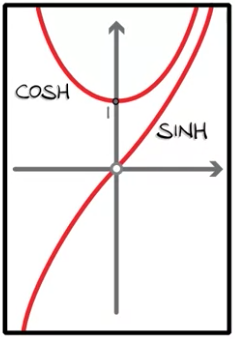
\includegraphics[width=4cm]{hyperbolic_trigs.png}
    \label{fig:hyperbolic_trigs}
\end{figure}

$$\cosh^2 - \sinh^2 = 1$$

\subsection{$\cosh{x}$}

\begin{equation}
\begin{split}
\cosh{x} & = \frac{e^x + e^{-x}}{2} \\
 & = \frac{1}{2}e^x + \frac{1}{2}e^{-x} \\
 & = \frac{1}{2}(1 + x + \frac{1}{2!}x^2 + \frac{1}{3!}x^3 + \frac{1}{4!}x^4 + \cdots) + \frac{1}{2}(1 - x + \frac{1}{2!}x^2 - \frac{1}{3!}x^3 + \frac{1}{4!}x^4 - \cdots) \\
 & = \Sigma_{k=0}^\infty \frac{x^{2k}}{(2k)!}
\end{split}
\end{equation}

\subsection{$\sinh{x}$}

\begin{equation}
\begin{split}
\cosh{x} & = \frac{e^x - e^{-x}}{2} \\
 & = \frac{1}{2}e^x - \frac{1}{2}e^{-x} \\
 & = \frac{1}{2}(1 + x + \frac{1}{2!}x^2 + \frac{1}{3!}x^3 + \frac{1}{4!}x^4 + \cdots) - \frac{1}{2}(1 - x + \frac{1}{2!}x^2 - \frac{1}{3!}x^3 + \frac{1}{4!}x^4 - \cdots) \\
 & = \Sigma_{k=0}^\infty \frac{x^{2k+1}}{(2k+1)!}
\end{split}
\end{equation}

\section{Principle}

\begin{equation}
\begin{split}
\frac{d}{dx}\sinh{x} & = \frac{d}{dx}\Sigma_{k=0}^\infty\frac{x^{2k+1}}{(2k+1)!} \\
 & = \Sigma_{k=0}^\infty(2k+1)\frac{x^{2k}}{(2k+1)!} \\ 
 & = \Sigma_{k=0}^\infty\frac{x^{2k}}{(2k)!} \\ 
 & = \cosh{x}
\end{split}
\end{equation}

\begin{equation}
\begin{split}
\frac{d}{dx}\cosh{x} & = \frac{d}{dx}\Sigma_{k=0}^\infty\frac{x^{2k}}{(2k)!} \\
 & = \Sigma_{k=1}^\infty(2k)\frac{x^{2k-1}}{(2k)!} \\ 
 & = \Sigma_{k=0}^\infty\frac{x^{2k+1}}{(2k+1)!} \\ 
 & = \sinh{x}
\end{split}
\end{equation}

\section{H.O.T}
Higher Order Terms

$$e^x = 1 + x + \frac{1}{2!}x^2 + \frac{1}{3!}x^3 + \frac{1}{4!}x^4 + \frac{1}{5!}x^5 + H.O.T$$

\subsection{Example: $f(x) = 1 - 2xe^{\sin{x^2}}$ }

$$sin{x^2} = x^2 - \frac{1}{3!}(x^2)^3 + H.O.T = x^2 - \frac{1}{6}x^6 + H.O.T$$

\begin{equation}
\begin{split}
e^{\sin{x^2}} & = 1 + (x^2 - \frac{1}{6}x^6 + H.O.T) + \frac{1}{2}(x^2 + H.O.T)^2 + \frac{1}{6}(x^2 + H.O.T)^3 + H.O.T \\
 & = 1 + x^2 + \frac{1}{2}x^4 + H.O.T \\
\end{split}
\end{equation}

\begin{equation}
\begin{split}
f(x) & = 1 - 2x(1 + x^2 + \frac{1}{2}x^4 + H.O.T) \\
 & = 1 - 2x - 2x^3 - x^5 + H.O.T
\end{split}
\end{equation}

\end{document}